% EN48 c05 | 原书 p.70–81（PDF 79–90） | 第 3 章（无小节）
% 边界：本章自原书 p.70 章首起，至 p.81 最后一条结果收尾；第 4 章自 p.82 起。
\section{阿贝尔簇 $V$ 与 $\Vdual$ 的同调镜像对称}

% ===== 原书 p.70 =====
环面的 SYZ 镜像属于族 Floer 理论（Family Floer theory）的一个例子 [Fuk02]。特别地，
族 Floer 理论表明，线丛应当镜像拉格朗日（子流形）的行为。原因在于：由 Serre 对偶有
$\mathrm{Ext}^1(\OO_{p_0},\OO)\iso\OO_{p_0}$，而环面上竖直的线性拉格朗日（子流形）
与任意其他有限斜率的线性拉格朗日（子流形）恰交于一点。我们可以对每个点定义一个
线丛，使之对应 Floer 理论一侧由该交点生成的一维向量空间；再在所得对象上赋予全纯
结构，即得全纯线丛，参看 [Fuk02]。由于 $\LL_{pt}$ 与有限斜率的线性拉格朗日（子流形）
恰有一个交点，我们可以由此构造一个秩 $1$ 的线丛。

\transnote{$\mathrm{Ext}^1(\OO_{p_0},\OO)\iso\OO_{p_0}$ 是 Serre 对偶的具体形态：
阿贝尔曲面上「点层」的一阶扩张仍是一维的。正因每个交点只贡献一维，交点个数才恰好
等于线丛一侧的态射维数。这也是下文把「交点生成的向量空间」当作纤维的动机。}

\medskip\noindent\textbf{深谷范畴 $\mathrm{Fuk}(\Vdual)$}\par

我们考虑深谷范畴 $\mathrm{Fuk}(\Vdual)$（一个 $A_\infty$-范畴）的如下全子范畴。

\begin{itemize}[leftmargin=2.2em,itemsep=0.25em]
\item 对象：令 $M=\begin{pmatrix}2&1\\1&2\end{pmatrix}$，$\Gamma_B:=M(\Z^2)$。在
  $v_0\colon Y\to\C$ 的纤维 $\Vdual$ 上有仿射作用--角坐标（affine action-angle
  coordinates）$(\xi_1,\xi_2,\theta_1,\theta_2)$，其中 $\xi_i$ 关于复坐标的范数单调，
  $\theta_i$ 是相应的辐角。在这些坐标下，纤维上的辛形式为 $\omega=\de\xi\wedge\de\theta$。
  我们考虑以如下线性拉格朗日（子流形）为对象的子范畴：
\[
\ell_i=\bigl\{(\xi_1,\xi_2,-i\cdot M^{-1}(\xi))\bigr\}_{\xi\in T_B=\R^2/M(\Z^2)}.
\]
  这些对象是 [PZ98] 中椭圆曲线上斜率 $i$ 的直线的类比。
\item 态射：设 $|i-j|\ge1$，则
  $\Hom(\ell_i,\ell_j):=\bigoplus_{p\in\ell_i\cap\ell_j}\C\cdot\{p\}\iso\C^{(i-j)^2}$，
  论证是模算术（modular arithmetic）的。注意这等于 $j>i$ 时的
  $h^0(V,\LL^{\otimes(j-i)})$，而 $i>j$ 时为 $h^2(V,\LL^{\otimes(j-i)})$；
  后一事实将告诉我们各态射群同构。若 $\xi$ 是 $\ell_i$ 上的坐标、$\tilde\xi$ 是
  $\ell_j$ 上的坐标，则交点只能出现在满足下式处：

% ===== 原书 p.71 =====
\begin{equation}\label{eq:3-1}
\begin{gathered}
1)\ \xi\equiv\tilde\xi\mod M(\Z^2)\\
2)\ i\cdot M^{-1}(\xi)\equiv j\cdot M^{-1}(\tilde\xi)\mod\Z^2\\
\Longrightarrow\ i\cdot\xi\equiv j\cdot\tilde\xi\equiv j\cdot\xi\mod M(\Z^2)\\
\Longrightarrow\ \xi\in\frac{1}{i-j}M(\Z^2)
\end{gathered}
\end{equation}
  于是令 $\xi=s(2,1)+t(1,2)$。此时 $(i-j)s$ 与 $(i-j)t$ 可取 $0$ 到 $i-j-1$ 之间的
  任意值，于是得到 $(i-j)^2$ 个交点。
\item $\hom$ 上的 $\mu^1$：微分计数交点之间的全纯双边形（bigon）。
\end{itemize}

\transnote{式~\eqref{eq:3-1} 的推导只用到一个事实：$M$ 是整矩阵。由 1) 知
$j\xi\equiv j\tilde\xi\pmod{M(\Z^2)}$；由 2) 乘以 $M$ 得
$i\xi\equiv j\tilde\xi\pmod{M(\Z^2)}$。两式相减得 $(i-j)\xi\in M(\Z^2)$，即
$\xi\in\frac{1}{i-j}M(\Z^2)$。该有限子群在 $T_B$ 中恰有 $(i-j)^2$ 个元素，
这正是交点数。}

\begin{claim}\label{claim:no-bigons}
对 $i\ne j$，$T^4$ 上线性拉格朗日子流形 $\ell_i\cap\ell_j$ 的任意两个交点之间都
没有双边形，因此 $\mu^1=0$。
\end{claim}

\begin{proof}
由偶对 $(T^4,\ell_i\cup\ell_j)$ 有
\[
0=\pi_2(T^4)(=\pi_2(\R^4))\to\pi_2(T^4,\ell_i\cup\ell_j)\to\pi_1(\ell_i\cup\ell_j)
\xrightarrow{\ \sim\ }\pi_1(T^4),
\]
故 $\pi_2(T^4,\ell_i\cup\ell_j)$ 平凡。于是任何这样的全纯盘都是可缩的。取 $T^4$ 上
以 $\ell_i\cup\ell_j$ 为边界、连接交点 $p,q$ 的双边形
$u\colon D^2\setminus\{\pm1\}\to T^4$。取提升 $\tilde\ell_i,\tilde\ell_j$，使提升后的
交点 $\tilde p=0$：
\[
\tilde\ell_i=\bigl\{(\xi_1,\xi_2,i\cdot M^{-1}(\xi))\bigr\}_{\xi\in\R^2}.
\]
设 $\partial_1,\partial_2$ 是 $D^2\setminus\{\pm1\}$ 的两个边界分支，分别映到
$\ell_i,\ell_j$。把 $u(\partial_i)$ 提升到 $\R^4$，记作 $\gamma_1,\gamma_2$，使
$\gamma_i(0)=\tilde p$，并令 $\tilde q_i:=\gamma_i(1)$。由盘的可缩性，
$\tilde q_1=\tilde q_2$。然而
\[
\tilde\ell_i\cap\tilde\ell_j
\Longrightarrow \xi^{(i)}=\xi^{(j)}=:\xi,\qquad i\xi=j\xi\ \therefore\ \xi=0,
\]
因为 $|i-j|\ge2$。所以至多只有一个交点，而非非平凡双边形所需的两点。
\end{proof}

% [Tutor Note: 断言只假设 i ≠ j，此处证明却用 |i−j| ≥ 2；当 |i−j| = 1 时由
% (i−j)ξ = 0 同样得 ξ = 0，结论不受影响。原书如此，保留。]

\transnote{证明的关键是「可缩」二字：盘可缩，故两个边界分支的端点提升后必须重合。
若存在非平凡双边形，两个端点应给出两个不同的交点，与唯一性矛盾。注意此处
$\tilde\ell_i$ 与 $\tilde\ell_j$ 是 $\R^4$ 中的平面，等式 $i\xi=j\xi$ 中的乘法是
数乘而非模运算，这正是可取 $\xi=0$ 的原因。}

% ===== 原书 p.72 =====
对相异的 $i,j$，态射空间维数为 $(i-j)^2$；仅当 $j>i$ 时它与
$h^0(V,\LL^{j-i})$ 相符，否则这些态射处于 Floer 次数 $2$，与
$h^2(V,\LL^{j-i})$（负线丛）相符。

另一方面，$i=j$ 时，$\ell_i$ 与它的小哈密顿扰动之间通常确实存在双边形。尽管如此，
$HF(\ell_i,\ell_i)=H^*(T^2)$ 仍然成立；所依赖的关键几何事实是 $\ell_i$ 在环面内
不围出任何盘，故自 $HF$ 约化为经典上同调。

若 $i=j$，由 PSS 同构（PSS isomorphism）有
$CF^*(\ell_i,\ell_i)=HF^*(\ell_i,\ell_i)$。于是
$HF^*(\ell_i,\ell_i)\iso H^*(\ell_i)=H^*(T^2)$。因此所有情形下都有
$HF^*(\ell_i,\ell_j)\iso\mathrm{Ext}^*_V(\LL^{\otimes i},\LL^{\otimes j})$。

\transnote{「不围出盘」为何足以让自 $HF$ 退化为经典上同调：没有盘，就不存在连通
两个交点的伪全纯盘，微分 $\mu^1$ 消失；再取哈密顿量为 Morse 函数并作小扰动，
Floer 复形便与奇异上同调同构。这也解释了 $i=j$ 时虽然有双边形、但 $\mu^1$ 仍可
取零的微妙之处：那些双边形在扰动极限下成对抵消。}

\begin{itemize}[leftmargin=2.2em,itemsep=0.25em]
\item 复合，即 $\hom$ 上的 $\mu^2$（与 [PZ98] 中椭圆曲线的图景类比）：我们考虑
  提升 $\tilde\ell_0,\tilde\ell_1,\tilde\ell_2$，考察可能出现的三角形。所得结果是
  一个以 $\Gamma$ 中元素为下标的和式，与多 $\theta$ 函数（multi-theta functions）
  的展开相符。
\item 单位态射：$\hom(\ell_i,\ell_i)\iso H^*(V,\ell_i)$，它自然带有单位元，但我
  认为这还需要更多工作。通常的做法是证明它同构于 Morse 复形（Morse complex）：
  取哈密顿量为 Morse 函数，然后考察 $\de f$。临界点对应 $\de f=0$ 处，在 Floer
  框架中给出交点；Morse 轨道也是常 $t$ 的 Floer 轨道，在这个特殊情形下 Floer
  方程与 Morse 方程恰好一致。哈密顿扰动在纤维内有效，尽管后文会看到它在全空间内
  无效。
\end{itemize}

% [Tutor Note: 原文写作 hom(ℓi, ℓi) ≅ H*(V, ℓi)，把拉格朗日 ℓi 当作「V 上的层」
% 来写上同调，记号略欠严格；按上下文应为 H*(ℓi)。保留原样。]

\medskip\noindent\textbf{有界导出范畴 $\DBCoh(V)$}\par

\begin{definition}\label{def:bounded-derived}
有界导出范畴（bounded derived category）的定义如下。令 $\cA$ 为 $V$ 上相干层
构成的范畴。注意 $V$ 是阿贝尔簇，从而是射影簇。
\end{definition}

\begin{claim}\label{claim:A-abelian}
$\cA$ 是阿贝尔范畴，特别地有核与余核，因此可以定义对象的链复形。
\end{claim}

\begin{definition}\label{def:kom}
令 $\mathrm{Kom}(\cA)$ 为 $\mathrm{Coh}(V)$ 中链复形构成的范畴，态射为链映射，
复合为链映射的复合。
\end{definition}

% [Tutor Note: 上一段应写「A 中链复形」；原文误写 Coh(V)，且此处 A 与 Coh(V) 本应
% 是同一范畴。保留原样。]

\begin{definition}\label{def:k-category}
令 $K(\cA)$ 的对象为如上链复形，态射则在同伦等价这一等价关系 $\sim$ 下等同。
\end{definition}

\begin{definition}\label{def:derived}
导出范畴 $D(\cA)$ 与 $K(\cA)$ 有相同的对象；态射 $A^\bullet\to B^\bullet$ 是一个
roof $A^\bullet\leftarrow C^\bullet\to B^\bullet$，其中 $C^\bullet\to A^\bullet$
是拟同构（quasi-isomorphism），即在上同调上诱导同构的链映射。若两个态射在
$K(\cA)$ 中同为第三个体所支配，则它们等价。
\end{definition}

% [Tutor Note: 「被第三个体所支配」原文作 dominated in K(A) by a third object of the
% same sort，这是导出范畴局部化的标准构造，但原文未给出「支配」的精确定义。保留原样，
% 读者可按 [Wei94, §10.4] 的 roof 等价关系理解。]

于是以 $\mathrm{Kom}^{\mathrm{b}}(\cA)$ 为起点执行上述过程，即只取有界链复形
（在有限多个对象之外为零），便得到有界导出范畴。

\begin{claim}\label{claim:dg-enhance}
$\DBCoh(V)$ 可以提升为 dg-范畴（dg-category），即满足 $\mu^{\ge3}=0$ 的
$A_\infty$-范畴。
\end{claim}

\transnote{「提升为 dg-范畴」指：除了上同调层面的态射群，还给每个态射空间配上
链复形结构以及满足结合律的复合，使同伦范畴恰好是导出范畴。$\mu^{\ge3}=0$ 表示
只有 $\mu^1$（微分）与 $\mu^2$（复合），故不必处理高阶运算，这正是导出范畴
「是 dg-范畴」的意思。}

% ===== 原书 p.73 =====
此处我们不需要这一点，因为在我们的设定中深谷范畴上 $\mu^1=0$，故可以证明普通
范畴之间的等价。

\begin{claim}\label{claim:split-generate}
回忆此前定义的 $\LL\to V$。我们断言 $\OO,\LL,\LL^2$ 分裂生成（split-generate）
$\DBCoh(V)$。
\end{claim}

\begin{remark}\label{rem:higher-products}
这使我们只需考虑这些对象，但代价是需要关于更高 $A_\infty$ 积的更多信息。原因是
其他对象将作为由 $\OO,\LL,\LL^2$ 构造的复形出现，而计算这些复形之间上同调层面的
$\hom$ 需要知道 $\OO,\LL,\LL^2$ 之间某些链层面的更高复合。特别地，原则上需要知道
所有涉及从 $\OO,\LL,\LL^2$ 中任取的对象序列的 $\mu^k$，且这些对象可任意重复。
\end{remark}

\begin{claim}\label{claim:ample}
如上定义的 $\LL$ 是丰富线丛（ample line bundle）。
\end{claim}

\begin{proof}
复环面上的线丛由 Hermite 形式 $H$ 刻画（见 Polishchuk 关于阿贝尔簇的书 [Pol03]）。
丰富线丛等价于存在某个 $i$ 使 $H^0(V,\LL^i)\ne0$；本设定正是如此，因为 $i>0$ 时
$\LL^i$ 有 $i^2$ 个截面。此外，映射 $V\ni x\mapsto t_x^*\LL\otimes\LL$ 的核有限，
这等价于 $H$ 非退化（见 [Pol03, 第 8.5--8.6 章]）。但此处
\[
H=\begin{pmatrix}2&1\\1&2\end{pmatrix}
\]
行列式非零，即非退化，故 $\LL$ 丰富，断言成立。
\end{proof}

\begin{corollary}\label{cor:projective}
阿贝尔簇 $V$ 是射影的。
\end{corollary}

为给出分裂生成的定义，先作一些准备。

\begin{definition}\label{def:triangulated}
若范畴 $\cC$ 包含所有映射锥（mapping cone），即对任意态射 $f$，对象
$\mathrm{Cone}(f)$ 是 $\cC$ 中的对象，则称 $\cC$ 是三角的（triangulated）。更
准确地说，它包含平移函子（shift functor），即自等价 $A\mapsto A[1]$，并带有一类
distinguished triangles。
\end{definition}

\begin{definition}\label{def:thick}
三角子范畴 $\cD\subset\cC$ 称为厚的（thick），若它对取直和项封闭，即
$E\oplus F\in\mathrm{Ob}(\cD)\Longrightarrow E,F\in\mathrm{Ob}(\cD)$。
\end{definition}

\begin{definition}\label{def:split-generate}
若一组对象 $\{G_i\}_{i\in I}\in\mathrm{Ob}(\cC)$ 的厚包络（thick envelope）是
$\cC$，即取包含诸 $G_i$ 且对取直和项封闭的最小三角范畴得到整个 $\cC$，则称它们
分裂生成 $\cC$。
\end{definition}

\begin{proof}[断言~\ref{claim:split-generate} 的证明]
以下论证来自 MSRI 导出范畴暑期学校 [APS, 第 5.3 讲]。每个复形由其上的上同调生成，
故只需证明任意相干层 $F$ 落在 $\OO,\LL,\LL^2$ 的厚包络中；这样 $\DBCoh(V)$ 的
每个元素都会被厚包络达到，换言之 $\OO,\LL,\LL^2$ 分裂生成。

% ===== 原书 p.74 =====
我们已看到 $V$ 是射影的，因而 $\mathrm{Coh}(V)$ 有足够多的局部自由层（文献）。
特别地，$n$ 充分大时 $F(n)$ 由整体截面生成，即有满射
$\OO_X^n\twoheadrightarrow F(n)$；于是扭以 $\OO(-n)$、并对
$\OO_X(-n)^n\to F$ 的核重复此过程，便得到 $F$ 的局部自由消解：
\[
\cdots\to P^{-N}\to P^{-N+1}\to\cdots\to P^0\to F\to0.
\]
令 $Q$ 为截断至次数 $N$ 所得的复形：
\[
Q:=[P^{-N}\to\cdots\to P^{-1}\to P^0].
\]
则 $Q$ 落在厚包络 $\langle\OO,\LL,\LL^2\rangle$ 中，因为所有 $P^i$ 都以 $\LL^i$
为直和项，而 $\langle\OO,\LL,\LL^2\rangle$ 是完全例外收集体（full exceptional
collection）（文献），包含 $\LL$ 的所有幂。有复形的包含 $P^\bullet\to Q$，其商为
\[
G[N+1]=\cdots\to P^{-N-1}\to0\to0\cdots\to0,
\]
其中 $G$ 定义为次数 $-N-1$ 的上同调，因为复形其余部分正合。特别地，$G$ 是相干层，
且得到态射
\[
F\to G[N+1]\in\mathrm{Ext}^{N+1}(F,G)\iso
\mathrm{Ext}^{2-N-1}(G,F\otimes\omega)^*=0,
\]
最后一步用 Serre 对偶。于是有
\[
G[N]\longrightarrow Q\longrightarrow F\xrightarrow{\ 0\ }G[N+1],
\]
由此 $Q\iso G[N]\oplus F$。已知 $Q$ 在厚包络中，而厚包络对直和项封闭，故 $F$ 也
在其中，证毕。
\end{proof}

\transnote{此证明是本章的技术核心，可拆成三步读。其一，用射影性得到局部自由消解，
把 $F$ 换成有限复形 $Q$；其二，用 Serre 对偶把 $\mathrm{Ext}^{N+1}(F,G)$ 消成零，
从而让短正合列分裂，得到 $Q\cong G[N]\oplus F$；其三，厚包络对直和项封闭，于是
$F$ 作为 $Q$ 的直和项也在其中。三步缺一不可。}

因此，只需在 $\OO,\LL,\LL^2$ 上考察函子，即可证明范畴的全忠实嵌入，代价是需要
知道更高的 $A_\infty$ 积。

\medskip\noindent\textbf{走向 HMS：全忠实嵌入
$\DBCoh(V)\hookrightarrow\mathrm{Fuk}(\Vdual)$}\par

函子 $\DBCoh(V)\to\mathrm{Fuk}(\Vdual)$ 如下。在对象上，
$\LL^{\otimes k}\mapsto\ell_k$。回忆 §1.2 的基公式（原书 1.2.17）：$H^0(V,\LL^{\otimes l})$ 有以下
截面基：
\[
s_{e,l}:=\sum_\gamma\tau^{-l\kappa(\gamma+\frac{\gamma_{e,l}}{l})}
x^{-l\lambda(\gamma)-\gamma_{e,l}}.
\]

% [Tutor Note: 原书此式末项印作 −γ_{e,l}，漏写 λ；按原书 1.2.17 以及本页下方乘积
% 公式，正确形式应为 x^{−λ(lγ+γ_{e,l})}，即指数末项为 −λ(γ_{e,l})。此处照原书排印，
% 不作改动。]

\transnote{上式指数末项在原书三处排印不一：p.74 印作
$-\gamma_{e,l}$，p.77 的同一基印作 $x^{-\lambda(l\gamma-\gamma_{e,l})}$，而原书
1.2.17 印作 $x^{-l\lambda(\gamma)-\lambda(\gamma_{e,l})}$。三者中只有最后一式
（等价于 $x^{-\lambda(l\gamma+\gamma_{e,l})}$）与下面的乘积公式自洽。阅读时以
原书 1.2.17 为准。}

% ===== 原书 p.75 =====
其中 $\gamma_{e,l}=s\gamma'+t\gamma''$，$0\le s,t<l$。于是在态射上，函子的作用
如下（$s_i$ 记 $\gamma_{e,l}$ 的各种取法）：
\begin{align*}
\hom(\OO,\LL)=H^0(V,\LL)\ni s&\mapsto
p\in\hom(\ell_0,\ell_1)=\bigoplus_{p\in\ell_0\cap\ell_1}\C\cdot p=\C\cdot p,\\
\hom(\OO,\LL^2)=H^0(V,\LL^2)\ni(s_1,s_2,s_3,s_4)&\mapsto
(p_1,p_2,p_3,p_4)\in\bigoplus_{p\in\ell_0\cap\ell_2}\C\cdot p,\\
&\qquad\text{此处 }|\ell_0\cap\ell_2|=4,\\
\hom(\LL,\LL^2)\iso\hom(\OO,\LL^*\otimes\LL^2)&\iso\hom(\OO,\LL)
=H^0(V,\LL)\\
&\qquad\ni s\mapsto p'\in\hom(\ell_1,\ell_2)=\C\cdot p'.
\end{align*}
与复合相容，即：
\begin{gather*}
s(x)=\sum_\gamma\tau^{-\kappa(\gamma)}x^{-\lambda(\gamma)},\qquad
s^2(x)=\sum_{\tilde\gamma,\tilde{\tilde\gamma}}
\tau^{-\kappa(\tilde\gamma)-\kappa(\tilde{\tilde\gamma})}
x^{-\lambda(\tilde\gamma)-\lambda(\tilde{\tilde\gamma})},\\
\hom(\LL,\LL^2)\otimes\hom(\OO,\LL)\ni s^2(x)=c_1s_1+c_2s_2+c_3s_3+c_4s_4\\
\longleftrightarrow\ \mu^2(p,p')=c_1p_1+c_2p_2+c_3p_3+c_4p_4.
\end{gather*}
特别地，我们预期系数 $c_i$ 是某个特定 $x$ 值的 $\theta$ 函数 $s(x)$，类比
[PZ98] 的计算。我们希望用 $H^0(V,\LL^2)$ 的这组基表示 $s^2(x)$。把 $s^2(x)$ 的
和式按 $\tilde\gamma+\tilde{\tilde\gamma}$ 中 $(\gamma',\gamma'')$ 系数对的四种
可能奇偶性拆成四个和。然后作坐标变换
\[
\gamma=\tfrac12(\tilde\gamma+\tilde{\tilde\gamma}-\gamma_e),\qquad
\eta=\tfrac12(\tilde{\tilde\gamma}-\tilde\gamma-\gamma_e),\qquad
\gamma_e\in\{0,\gamma',\gamma'',\gamma'+\gamma''\}.
\]
例如，若 $\tilde\gamma+\tilde{\tilde\gamma}=(n_1+m_1)\gamma'+(n_2+m_2)\gamma''$
且 $n_1+m_1$、$n_2+m_2$ 均为偶数，则可将 $\tilde\gamma+\tilde{\tilde\gamma}$ 写成
某个 $\gamma\in\Gamma_B$ 的 $2\gamma$。若二者一奇一偶，则须减去 $\gamma'$，等等。
这样得到 $\gamma_e$ 的四种取法。于是可按四种奇偶选择把 $s^2(x)$ 拆成四个和，
用诸 $s_i(x)$ 表示。

% ===== 原书 p.76 =====
再回忆二次型 $\kappa$ 满足
$\kappa(\gamma+\eta)=\kappa(\gamma)+\kappa(\eta)-\ip{\gamma}{\lambda(\eta)}$。
\begin{align*}
s^2(x)&=\sum_{\tilde\gamma,\tilde{\tilde\gamma}}
\tau^{-\kappa(\tilde\gamma)-\kappa(\tilde{\tilde\gamma})}
x^{-\lambda(\tilde\gamma+\tilde{\tilde\gamma})}\\
&=\sum_{\gamma,\eta}\Bigl[
\tau^{-\kappa(\gamma-\eta)-\kappa(\gamma+\eta)}x^{-2\lambda(\gamma)}\\
&\qquad+\tau^{-\kappa(\gamma+\gamma'/2-\eta-\gamma'/2)
-\kappa(\gamma+\gamma'/2+\eta+\gamma'/2)}x^{-2\lambda(\gamma)}x_1^{-1}\\
&\qquad+\tau^{-\kappa(\gamma+\gamma''/2-\eta-\gamma''/2)
-\kappa(\gamma+\gamma''/2+\eta+\gamma''/2)}x^{-2\lambda(\gamma)}x_2^{-1}\\
&\qquad+\tau^{-\kappa(\gamma+(\gamma'+\gamma'')/2-\eta-(\gamma'+\gamma'')/2)
-\kappa(\gamma+(\gamma'+\gamma'')/2+\eta+(\gamma'+\gamma'')/2)}
x^{-2\lambda(\gamma)}(x_1x_2)^{-1}\Bigr]\\
&=\sum_\eta\tau^{-2\kappa(\eta)}\sum_\gamma\tau^{-2\kappa(\gamma)}x^{-2\lambda(\gamma)}\\
&\qquad+\sum_\eta\tau^{-2\kappa(\eta+\gamma'/2)}\sum_\gamma
\tau^{-2\kappa(\gamma+\gamma'/2)}x^{-2\lambda(\gamma)}x_1^{-1}\\
&\qquad+\sum_\eta\tau^{-2\kappa(\eta+\gamma''/2)}\sum_\gamma
\tau^{-2\kappa(\gamma+\gamma''/2)}x^{-2\lambda(\gamma)}x_2^{-1}\\
&\qquad+\sum_\eta\tau^{-2\kappa(\eta+(\gamma'+\gamma'')/2)}
\sum_\gamma\tau^{-\kappa(\gamma+(\gamma'+\gamma'')/2)}x^{-2\lambda(\gamma)}
(x_1x_2)^{-1}\\
&=\sum_\eta\tau^{-2\kappa(\eta)}s_1
+\sum_\eta\tau^{-2\kappa(\eta+\gamma'/2)}s_2\\
&\qquad+\sum_\eta\tau^{-2\kappa(\eta+\gamma''/2)}s_3
+\sum_\eta\tau^{-2\kappa(\eta+(\gamma'+\gamma'')/2)}s_4.
\end{align*}

\transnote{这一段只做了一件事：把 $s^2(x)$ 按 $\gamma_e\in\{0,\gamma',\gamma'',
\gamma'+\gamma''\}$ 分成四组，再用 $\kappa$ 的极化恒等式把每组的指数化成
「只含 $\eta$ 的因子 × 只含 $\gamma$ 的因子」。四组的 $\eta$ 因子恰是四个
$\tau$ 级数，$\gamma$ 因子恰是四个加权的 $s_i$，于是 $s^2(x)=\sum_i C_i s_i$。
四个系数 $C_i$ 正是后面要数三角形的对象。}

\begin{claim}\label{claim:coeff-triangle}
诸 $s_i$ 上的系数与三角形计数相符，即与深谷范畴中的 $\mu^2$ 相符。
\end{claim}

\begin{proof}
用 $\tilde{\ }$ 记到万有覆盖 $\R^4$ 的提升。把 $\tilde\ell_0\cap\tilde\ell_2$
放在三角形中的位置有四种选择（其他选择在阿贝尔簇上给出相同的三角形）。由
式~\eqref{eq:3-1} 的计算，取
\[
\tilde p_e=(\gamma_e/2,2M^{-1}(\gamma_e/2))=(\gamma_e/2,\lambda(\gamma_e)),
\]
因为 $\lambda$ 是线性映射 $M^{-1}$。已知 $p=\ell_0\cap\ell_1$ 的提升 $\tilde p$
必落在过 $\tilde p_e$ 的 $\tilde\ell_0$ 上。沿 $\tilde\ell_0$ 后两个坐标不变，
故 $\lambda(\gamma_e)$ 就是角坐标；又 $\tilde p$ 位于 $(0,0)$ 之上，故第一个坐标
是某个 $\eta\in\Gamma_B$：
\[
\tilde p=(\eta,\lambda(\gamma_e)).
\]
若 $\tilde p$ 位于 $(0,0)$，则 $p'=\ell_1\cap\ell_2$ 的提升是某个
$(\xi,M^{-1}(\xi))=(\xi,\lambda(\xi))$，因为 $\tilde\ell_2$ 会过原点（设拉格朗日
按顺时针排列）。由于它可能被 $(\eta,\lambda(\gamma_e))$ 平移，得到
$\tilde p'=(\eta,\lambda(\gamma_e))+(\xi,\lambda(\xi))$，其中 $\xi$ 由
$\overrightarrow{\tilde p'\tilde p_e}$ 落在 $\tilde\ell_2$ 上确定，即角度改变
$2\lambda$：
\[
\overrightarrow{\tilde p'\tilde p_e}
=\ip{\eta+\xi-\gamma_e/2}{\lambda(\gamma_e+\xi)-\lambda(\gamma_e)}
\]
\[
\Longrightarrow\ 2\lambda(\eta+\xi-\gamma_e/2)=\lambda(\xi)
\ \therefore\ \xi=\gamma_e-2\eta,\qquad
\therefore\ \tilde p'=(\gamma_e-\eta,2\lambda(\gamma_e-\eta)).
\]
\end{proof}

% ===== 原书 p.77 =====
\begin{figure}[htbp]
\centering
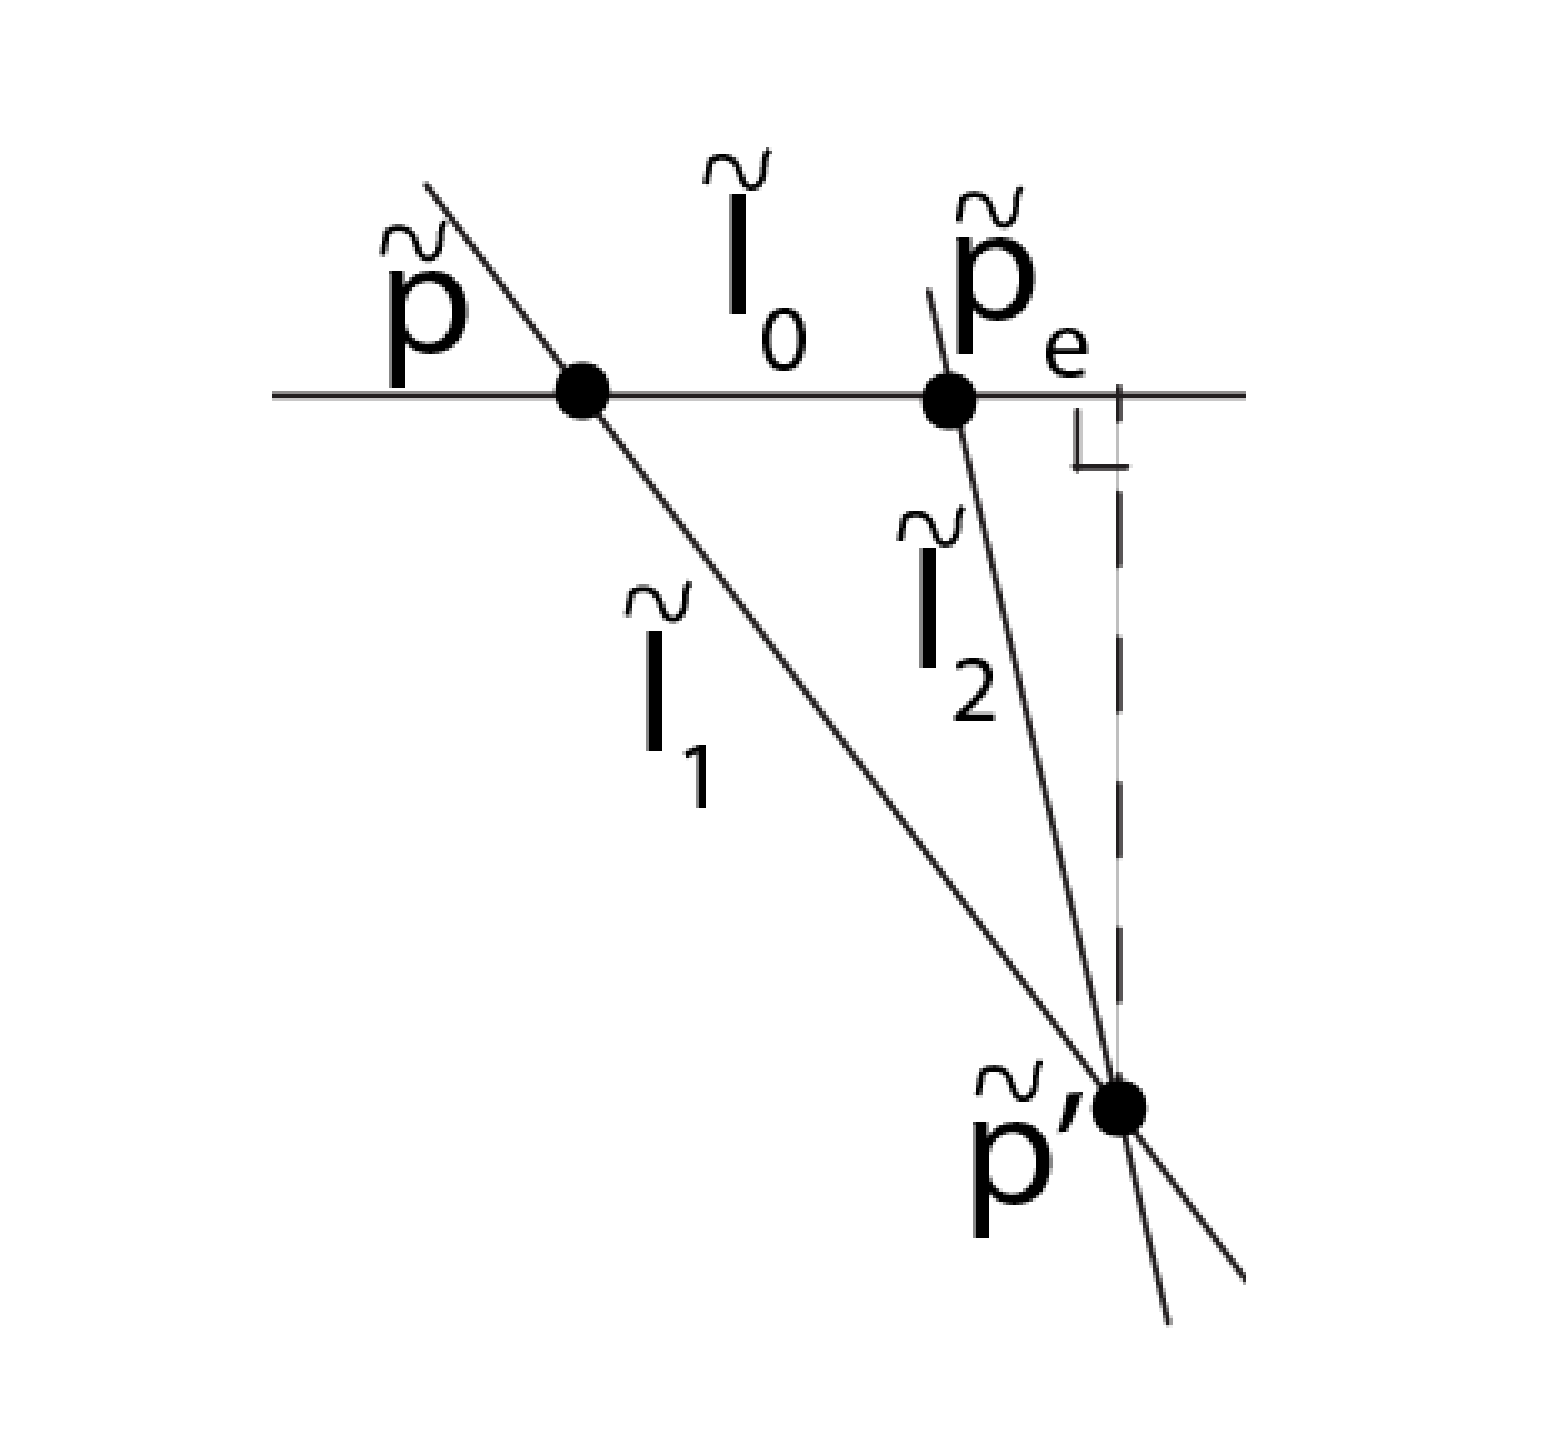
\includegraphics[width=0.42\textwidth]{figures/fig_3_1.png}
\caption{椭圆曲线情形中的三角形，以及 $T^4$ 情形的代表（原书 p.77）}
\label{fig:3-1}
\end{figure}

现在三角形已有三个点，我们要求它的面积。受椭圆曲线情形的图景启发（见图~\ref{fig:3-1}），
若把 $\tilde p_e$ 沿 $\tilde p_e$ 与 $\tilde p$ 的连线向远离 $\tilde p$ 的方向
延长同样的距离，便得到直角三角形。这可由三边构成勾股三元组看出：
\[
|\eta-\gamma_e/2|^2+|\lambda(\gamma_e-2\eta)|^2=(\text{第三边长})^2.
\]
于是取底边的一半与同样的高，得到三角形面积
\[
\frac12\int_\Delta\de\xi\wedge\de\theta
=\ip{(\eta-\gamma_e/2)}{\lambda(\eta-\gamma_e/2)}
=-2\kappa(\eta-\gamma_e/2).
\]
这与复侧 $\tau$ 的指数一致，断言证毕。

\transnote{面积公式把辛几何与复几何接了起来：左边是三角形在 $(\xi,\theta)$ 平面中
的辛面积，右边是二次型 $\kappa$ 在 $\eta-\gamma_e/2$ 处的取值。请注意 $\kappa$ 是
负定的（在第一 Chern 类的尺度下），故当 $\eta\ne\gamma_e/2$ 时右边为正，与面积
的符号一致；$-\!2\kappa$ 前面的负号正是由此而来。}

下面要证明乘法在更一般的情形 $i<j<k$ 下相符。先考虑线丛。有
$\Hom(\LL^i,\LL^j)\iso H^0(V,\LL^{j-i})$，故令 $l:=j-i$，$l':=k-j$。取
$\LL^l$ 的如下基：
\[
s_{e,l}:=\sum_\gamma\tau^{-l\kappa(\gamma+\frac{\gamma_{e,l}}{l})}
x^{-\lambda(l\gamma-\gamma_{e,l})}.
\]

% [Tutor Note: 与 p.74 的基是同一对象，原书此处印作 x^{−λ(lγ−γ_{e,l})}，括号内
% 符号应为 +（即 x^{−λ(lγ+γ_{e,l})}）。下方乘积公式与此不符时无法推出，故按原书
% 排印并加注；正确形式见原书 1.2.17。]

特别地，$\gamma_{e,l}=s\gamma'+t\gamma''$（$0\le s,t<l$），给出
$H^0(V,\LL^l)$ 的 $l^2$ 个基元素。我们希望用 $H^0(V,\LL^{l+l'})$ 的基表示两个
这样的截面之积，并把系数与另一侧的三角形计数比较。
\[
s_{e,l}\cdot s_{e,l'}=\sum_{\tilde\gamma,\tilde{\tilde\gamma}}
\tau^{-l\kappa(\tilde\gamma+\frac{\gamma_{e,l}}{l})
-l'\kappa(\tilde{\tilde\gamma}+\frac{\gamma_{e,l'}}{l'})}
x^{-\lambda(l\tilde\gamma+\gamma_{e,l}+l'\tilde{\tilde\gamma}+\gamma_{e,l'})}.
\]

% ===== 原书 p.78 =====
我们希望用 $H^0(V,\LL^{l+l'})$ 的类似基表示它：
\[
s_e:=\sum_\gamma\tau^{-(l+l')\kappa(\gamma+\frac{\gamma_e}{l+l'})}
x^{-(l+l')\lambda(\gamma+\frac{\gamma_e}{l+l'})}.
\]
把乘积中 $x$ 的幂与之比较，我们这样定义 $\gamma$：把和
$l\tilde\gamma+\gamma_{e,l}+l'\tilde{\tilde\gamma}+\gamma_{e,l'}$ 看作
$(l+l')\Gamma_B$ 中的元素加一个余项 $\gamma_e$。即令该元素为 $\gamma\in\Gamma_B$，
余项记为 $\gamma_e$：
\[
(l+l')\gamma+\gamma_e:=l\tilde\gamma+\gamma_{e,l}
+l'\tilde{\tilde\gamma}+\gamma_{e,l'}.
\]
类比上面的 $(i,j,k)=(0,1,2)$ 情形，我们希望用新变量 $A,B$ 作坐标变换，使 $\tau$
的指数满足等式
\[
\Bigl(\tilde\gamma+\frac{\gamma_{e,l}}{l},\ 
\tilde{\tilde\gamma}+\frac{\gamma_{e,l'}}{l'}\Bigr)
=\Bigl(A-\frac{B}{l},\ A+\frac{B}{l'}\Bigr),
\]
因为
$-l\kappa(A-\frac{B}{l})-l'\kappa(A+\frac{B}{l'})
=-(l+l')\kappa(A)-(\frac1l+\frac1{l'})\kappa(B)$。我们希望
$A=\gamma+\frac{\gamma_e}{l+l'}$，而它确实成立。$B$ 应当是变量 $\eta$ 与余项的
函数，使得 $\eta\in\Gamma_B$。我们作如下定义；它确实满足要求，其动机在下面的
三角形计数中会变得清楚：
\[
B=\frac{ll'}{l+l'}\Bigl(\tilde\gamma+\frac{\gamma_{e,l}}{l}
-\tilde{\tilde\gamma}-\frac{\gamma_{e,l'}}{l'}\Bigr)
=:\eta-\frac{l\gamma_e}{l+l'}.
\]

\begin{claim}\label{claim:eta-lattice}
$\eta\in\Gamma_B$。
\end{claim}

\begin{proof}
\[
\eta=\frac{ll'}{l+l'}\Bigl(\tilde\gamma+\frac{\gamma_{e,l}}{l}
-\tilde{\tilde\gamma}-\frac{\gamma_{e,l'}}{l'}\Bigr)+\frac{l\gamma_e}{l+l'}
\]
\[
=\frac{1}{l+l'}\bigl(ll'\tilde\gamma+l'\gamma_{e,l}
-ll'\tilde{\tilde\gamma}-l\gamma_{e,l'}-l(l+l')\gamma
+l^2\tilde\gamma+l\gamma_{e,l}+ll'\tilde{\tilde\gamma}+l\gamma_{e,l'}\bigr)
=l\tilde\gamma+\gamma_{e,l}-l\gamma\in\Gamma_B.
\]
\end{proof}

% [Tutor Note: 原书此证明以划掉符号标出相消的两项 ll′γ̃̃ 与 −lγ_{e,l′}，并靠
% l²γ̃ 与 l(l+l′)γ 两项合并。此处按展开式排印，划掉痕迹从略。]

\begin{corollary}\label{cor:product-basis}
\begin{align*}
s_{e,l}\cdot s_{e,l'}&=\sum_{\tilde\gamma,\tilde{\tilde\gamma}}
\tau^{-l\kappa(\tilde\gamma+\frac{\gamma_{e,l}}{l})
-l'\kappa(\tilde{\tilde\gamma}+\frac{\gamma_{e,l'}}{l'})}
x^{-\lambda(l\tilde\gamma+\gamma_{e,l}+l'\tilde{\tilde\gamma}+\gamma_{e,l'})}\\
&=\sum_{\gamma,\eta}\tau^{-l\kappa\bigl(\gamma+\frac{\gamma_e}{l+l'}
-\frac1l(\eta-\frac{l\gamma_e}{l+l'})\bigr)
-l'\kappa\bigl(\gamma+\frac{\gamma_e}{l+l'}+\frac1{l'}
(\eta-\frac{l\gamma_e}{l+l'})\bigr)}
x^{-(l+l')\lambda(\gamma)-\lambda(\gamma_e)}\\
&=\sum_\eta\tau^{-(\frac1l+\frac1{l'})\kappa(\eta-\frac{l\gamma_e}{l+l'})}
\sum_\gamma\tau^{-(l+l')\kappa(\gamma+\frac{\gamma_e}{l+l'})}
x^{-(l+l')\lambda(\gamma)-\lambda(\gamma_e)}.
\end{align*}
\end{corollary}

% ===== 原书 p.79 =====
\begin{claim}\label{claim:functor-composition}
左竖直函子 $\DBCoh(V)\to\mathrm{Fuk}(\Vdual)$ 与复合相容。
\end{claim}

\begin{proof}
我们把两个截面之积的表达式中的系数与三角形计数作比较。分别取 $p_1,p_2,p_3$ 为
$\ell_i\cap\ell_k$、$\ell_i\cap\ell_j$、$\ell_j\cap\ell_k$ 中的点。
$\ell_i\cap\ell_k$ 有 $(l+l')^2$ 种选择如下：
\[
p_1=\Bigl(\frac{\gamma_e}{k-i},-\frac{k}{k-i}\lambda(\gamma_e)\Bigr).
\]
则 $\overrightarrow{p_2p_1}$ 落在 $\tilde\ell_i$ 上，故形如
$(\xi,-i\lambda(\xi))$。又 $p_2$ 落在 $\ell_i$ 的提升上，故也是这种形式（我们用
$\eta/l$，使 $\eta\in\Gamma_B$ 最终与上面多 $\theta$ 函数中所用的 $\eta$ 一致），
至多相差一个格元素的平移，而该平移是 $(0,\lambda(\gamma_e))$：
\[
p_2=\Bigl(\frac\eta l,-i\lambda\Bigl(\frac\eta l\Bigr)-\lambda(\gamma_e)\Bigr),
\]
\[
\overrightarrow{p_2p_1}=\Bigl(\frac{\gamma_e}{k-i}-\frac\eta l,
-\frac{k}{k-i}\lambda(\gamma_e)+i\lambda\Bigl(\frac\eta l\Bigr)+\lambda(\gamma_e)\Bigr)
=(\xi,-i\lambda(\xi)).
\]
于是 $p_3(A,B)$ 有两个条件如下：
\begin{gather*}
\overrightarrow{p_2p_3}=\Bigl(A-\frac\eta l,
B+i\lambda\Bigl(\frac\eta l\Bigr)+\lambda(\gamma_e)\Bigr)\\
\therefore\ B+i\lambda\Bigl(\frac\eta l\Bigr)+\lambda(\gamma_e)
=-j\lambda\Bigl(A-\frac\eta l\Bigr)\\
\overrightarrow{p_1p_3}=\Bigl(A-\frac{\gamma_e}{k-i},
B+\frac{k}{k-i}\lambda(\gamma_e)\Bigr)\\
\therefore\ B+\frac{k}{k-i}\lambda(\gamma_e)
=-k\lambda\Bigl(A-\frac{\gamma_e}{k-i}\Bigr)
\Longrightarrow\ B=-k\lambda(A)\\
\Longrightarrow\ -k\lambda(A)=-j\lambda(A)+(j-i)\lambda\Bigl(\frac\eta l\Bigr)
-\lambda(\gamma_e)\\
\Longrightarrow\ (k-j)A=(i-j)\frac\eta l+\gamma_e\\
\therefore\ A=\frac{i-j}{k-j}\frac\eta l+\frac{1}{k-j}\gamma_e
=-\frac1{l'}\eta+\frac1{l'}\gamma_e,\qquad B=-k\lambda(A).
\end{gather*}
我们令 $\zeta:=-\frac\eta l+\frac{\gamma_e}{l+l'}$，因为这个表达式多处出现。为求
三角形的辛面积（在同伦不变性下相同，即对以这些点为顶点的任意全纯三角形相同），
我们取 $\frac12\int_P\de\xi\wedge\de\theta$，其中 $P$ 是由
\[
\vec a:=\overrightarrow{p_2p_1}
=\Bigl(\frac{\gamma_e}{l+l'}-\frac\eta l,
-i\lambda\Bigl(\frac{\gamma_e}{l+l'}-\frac\eta l\Bigr)\Bigr)
=(\zeta,-i\lambda(\zeta))
\]
张成的平行四边形；为定义另一向量 $\vec b:=\overrightarrow{p_1p_3}$，我们先化简
下面的表达式：
\[
-\frac1{l'}\eta+\frac1{l'}\gamma_e-\frac{\gamma_e}{l+l'}
=\frac{l}{l'}\Bigl(-\frac\eta l+\frac{\gamma_e}{l+l'}\Bigr)=\frac{l}{l'}\zeta.
\]

% ===== 原书 p.80 =====
于是定义
\[
\vec b:=\overrightarrow{p_1p_3}
=\Bigl(\frac{l}{l'}\zeta,-k\lambda\Bigl(\frac{l}{l'}\zeta\Bigr)\Bigr),
\]
因为我们已令 $\tilde\ell_k$ 过原点，故 $\tilde\ell_k$ 上的点以及与它平行的向量
都形如 $(\xi,-k\lambda(\xi))$。最后可以计算辛面积。
\begin{align*}
\frac12\int_P\de\xi\wedge\de\theta
&=\frac12(a_\xi\cdot b_\theta-a_\theta\cdot b_\xi)
=\frac12\Bigl\langle\zeta,-k\lambda\Bigl(\frac{l}{l'}\zeta\Bigr)\Bigr\rangle
-\frac12\Bigl\langle -i\lambda(\zeta),\frac{l}{l'}\zeta\Bigr\rangle\\
&=\Bigl(\frac{kl}{l'}-\frac{il}{l'}\Bigr)\kappa(\zeta)
=\frac{l+l'}{ll'}\kappa\Bigl(-\eta+\frac{l\gamma_e}{l+l'}\Bigr).
\end{align*}
我们得到与上面 $\tau$ 的指数相同的表达式，即
$-(\frac1l+\frac1{l'})\kappa(\eta-\frac{l\gamma_e}{l+l'})$，因为 $\kappa$ 是
偶函数。
\end{proof}

\transnote{$\frac12(a_\xi b_\theta-a_\theta b_\xi)$ 是平行四边形面积的一半，即
三角形的辛面积；这一步把向量运算换成 $\kappa$ 的取值。最后的表达式与
注~3.0.17 中 $\tau$ 的指数一致，故「三角形计数 = 截面乘积的系数」在一般
$i<j<k$ 情形也成立。}

注：把 $\eta$ 改名，以免与此前的 $\eta\ge\varphi(\xi)$ 冲突。后一个 $\eta$ 只在
$\widetilde Y$ 上有意义，不能下降到商。

\begin{claim}\label{claim:triangles-holomorphic}
上面描述的、以 $\ell_i,\ell_j,\ell_k$ 为界的三角形是全纯的。
\end{claim}

在证明之前，我们先回忆：在本文例子的设定下，拉格朗日 Floer 理论与 $J$ 的选取
无关（无论 $J$ 正则或一般），如下所述。

\begin{lemma}\label{lem:regular-j}
存在 $\omega$-相容近复结构构成的稠密集
$\cJ_{reg}\subset\cJ(Y,\omega)$，使得对所有满足适当拉格朗日边界条件的
$J$-全纯映射 $u\colon\mathbb{D}\to Y$，线性化 $\bar\partial$-算子 $D_u$ 都是
满射。
\end{lemma}

我们推迟到后面更一般地讨论正则性时给出该引理的证明。

\begin{lemma}\label{lem:independence-j}
在 $\Vdual$ 上，$J_1$ 与 $J_2$ 给出的计数 $\mu_2$ 相等。
\end{lemma}

\begin{proof}[略证]
这将依赖上一条陈述证明中的论证。论证相同，但我们的 Fredholm 问题在 Banach 丛的
配置中会多出一个 $[0,1]$ 因子，于是得到一维流形。预计没有其他边界，因为：
1) 球面泡发生在余维 $2$，不会出现在一维空间中；2) 条状断裂会断下一个双边形，
但环面上没有双边形——由参数平移的考虑以及维数/指标的理由（即所有交点指标相同，
而断裂条带的两段指标相差 $2$，参看 Morse 情形中流线的类比）；3) 盘泡不出现，
因为环面上的拉格朗日（子流形）不围出盘（取环面的万有覆盖后 $\pi_2$ 保持不变，
而后者没有 $\pi_2$）。由于一维流形的带符号边界为零，对正则的 $J_1,J_2$ 有
$\mathcal{M}(3\ \text{点},\text{同调类},J_1)
=\mathcal{M}(3\ \text{点},\text{同调类},J_2)$。正则道路的稠密集的存在性，与
上面关于正则 $J$ 存在性的证明类似。
\end{proof}

% ===== 原书 p.81 =====
现在可以证明上面计数的三角形对某个合适选取的正则 $J$ 是全纯的。

\begin{proof}[断言~\ref{claim:triangles-holomorphic} 的证明]
为计数三角形，我们选取最方便的 $J$。我们希望 $J$ 恰当地变换
$\partial_\xi$。若变动一个复坐标而保持另外两个不变，则不行，因为 $v_0$ 无法
保持不变，而它在纤维上应当不变。故改为变动一个复坐标，保持另一个复坐标与 $v_0$
不变。

取相对于 $\xi,\theta$ 坐标非对角的 $J$：其左下块与右上块分别为 $\lambda$ 与
$-\lambda^{-1}$，其中 $\lambda=\begin{pmatrix}2&1\\1&2\end{pmatrix}^{-1}$。
它与 $-I$ 的平方关系成立；可验证它是相容的，因为把来自
$\de\xi\wedge\de\theta$ 的标准辛形式与这个 $J$ 相乘，确实得到度量，即正定的。
取 $\Vdual$ 的万有覆盖，把所得线性空间分成两个平面的积：
$P:=\langle\zeta,\lambda(\zeta)\rangle$ 与辛正交补 $P^\omega$。特别地，按 $J$
的定义，$P$ 与 $P^\omega$ 都是 $J$-全纯平面。

然后我们证明上面那些三角形对这个 $J$ 是全纯的。这些三角形由 $\vec a$ 与
$\vec b$ 张成，而它们相差符号分别为 $(\zeta,0)\in\langle\partial_{\xi_i}\rangle_i$
与 $(0,\lambda(\zeta))\in\langle\partial_{\theta_i}\rangle_i$。于是 $\tilde\ell_i$
是一个积：在 $\zeta,\lambda(\zeta)$ 平面内是线性三角形，在辛正交补内是常值。
$\xi$ 方向与 $\theta$ 方向满足恰当的变量替换性质，因为 $\theta=-i\lambda(\xi)+c$。

既然可以在分量 $P$ 与 $P^\omega$ 中工作，在 $P$ 中我们有一个全纯盘，其中 $J$ 是
复结构（因为二维中每个近复结构都可积），并带有指定的拉格朗日边界条件，故由
Riemann 映射定理（Riemann mapping theorem）它唯一。又 $\tilde\ell_i$ 在
$P^\omega$ 中为常值，故三穿孔盘到该平面的投影的边界条件必须是常值。进一步的
推论是：由平面中的标准正则性论证，这些盘是正则的。
\end{proof}

% [Tutor Note: 原文「Take the J that is offdiagonal with λ = M^{−1}, −λ^{−1} in
% lower left and upper right」未明说哪一块在左下、哪一块在右上；此处按「左下 λ、
% 右上 −λ^{−1}」排印，与后文 θ = −iλ(ξ) + c 相容。保留原文的含糊。]

\begin{remark}\label{rem:soap-bubble}
与在每个分量上乘以 $i$ 的标准 $J_0$ 相比，这个 $J$ 有些不寻常。若把房间角落的
肥皂泡想象为面积最小的、即 $J_0$-全纯的曲面，它会被拉向角落顶点相当多。然而对
这里这个 $J$，面积最小的三角形是线性的。
\end{remark}

\transnote{这条注给出「选特殊 $J$」的直觉：通常的 $J_0$ 下，过三点的面积最小盘
会紧贴三角形的「顶点」弯曲；而对这里构造的 $J$，$P$ 本身是 $J$-全纯平面，
直线三角形直接落在 $P$ 中，故它就是全纯盘。于是计数三角形可以完全化为平面内的
线性问题。}
